% TODO: P2
% Your model: Flesh out your own approach, perhaps amplifying themes from the 'Prior lit' section.

% Data: Likely to be very detailed if the datasets are new or unfamiliar to the community, or if familiar datasets are being used in new ways.

\section{DeepReflect}\label{sec:deepreflect}
% ~1440 words ≈ ~11–12 paragraphs
% DeepReflect is designed to cater to two broad categories of users:
% 1. Users who frequently interact with LLMs for personal queries. 
% 2. Researchers interested in the large scale analysis and shift in psychosocial paradigms.

\subsection{System Design}
% Design is precise, methodical and shows some flair.


\textcolor{black!40}{Introduce. Mention that it has two key components - the analysis and the generation. Your model: Flesh out your own approach, perhaps amplifying themes from the 'Prior lit' section. Mention RQ1 from Section~\ref{sec:RQs} and put a figure depicting the system architecture with the 2 potential users (researchers, consumers / participants) here.}

% \textcolor{black!30}{AITAH judgments are used as a proxy for Empathy (Empathy, Active Listening, Non-judgmental Acceptance, and Unconditional Positive Regard, Emotional Safety) under the Rogerian paradigm and Sycophancy.}

\subsection{Evaluation Framework}

The evaluation framework consists of the following steps in a pipeline architecture (see Figure~\ref{fig:pipeline}):

\begin{figure}[h!]
    \centering
    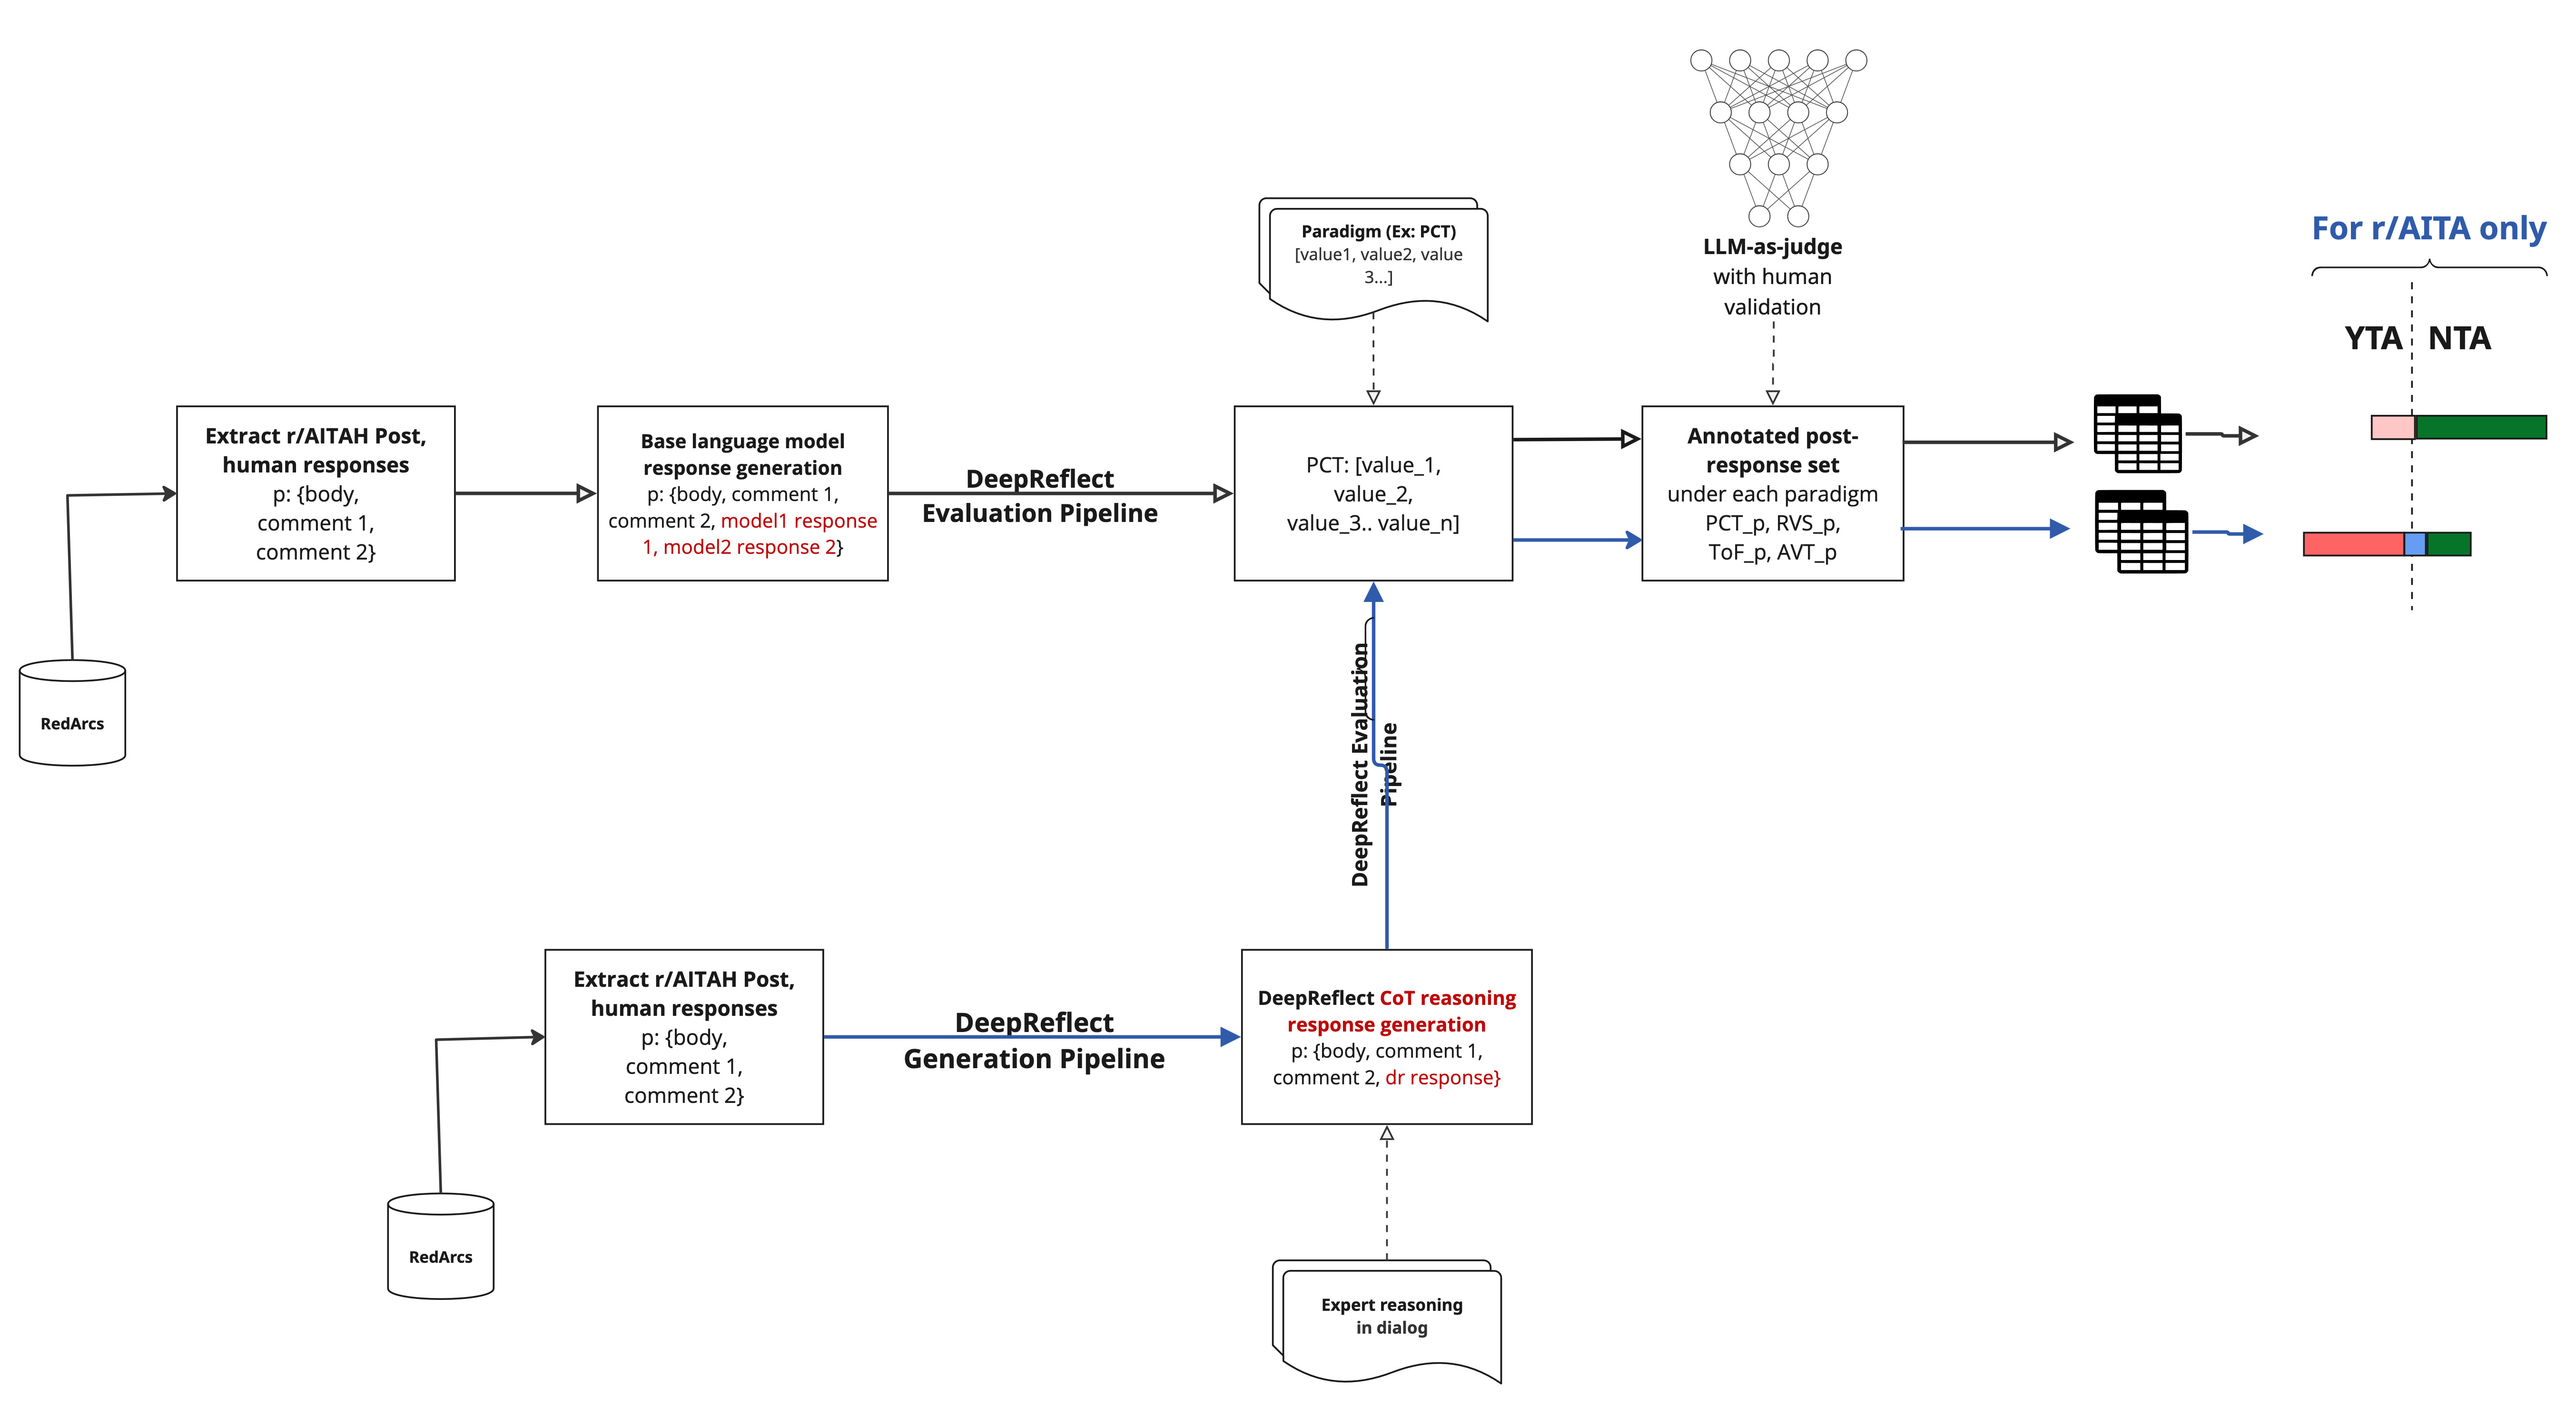
\includegraphics[width=0.98\columnwidth]{Diagrams/pipeline.jpg}
    \caption{Pipeline architecture for DeepReflect.}
    \label{fig:pipeline}
\end{figure}

\begin{enumerate}
    \item \textbf{Extract Posts}: Posts are extracted from two subreddits: (1) \texttt{r/AITAH} and (2) \texttt{r/Anxiety}. For each post, three components are considered: the body the original post written by the author (OP), the most upvoted human-written comment, and the comment with which the OP engaged the most. Further details regarding data filtering and text preprocessing are provided in Section~\ref{sec:Methods}.
    \item \textbf{Language Model Response Generation}: For each post and body, a baseline response is generated using a large language model (LLM) and appended to a table containing: (i) the model-generated responses, (ii) the top upvoted human comment, and (iii) the most engaged human comment (available for approximately half of the posts). The resulting dataset therefore consists of the original post body, paired with both human and AI responses.
    \item \textbf{Read psychosocial frameworks and corresponding set of values}: The following psychosocial frameworks are considered: (1) RVS, (2) Rogerian PCT, (3) Goffman’s ToF, and (4) Anthropic’s Value Tree. The frameworks are associated with distinct sets of values and behaviors as described in Section~\ref{sec:Litreview}. The frameworks are read into the system for annotations in the next step.
    \item \textbf{Feature Extraction and Annotation}: The LLM-as-a-judge paradigm \cite{zheng-et-al} is employed to annotate features for both the post body and each response under the 4 selected psychosocial paradigms. In this step, human validation is performed to calculate Cohen's Kappa and accuracy metrics to gauge the quality of the annotations.
    % Cohen's Kappa
    \[
    \kappa = \frac{p_o - p_e}{1 - p_e},
    \]
    \[
    \begin{aligned}
    p_o &= \text{observed agreement (accuracy)} \\
    p_e &= \text{expected agreement by chance}
    \end{aligned}
    \]
    See section~\ref{sec:Methods} for further details.
    \item \textbf{Save outputs to dataset}: The annotated data is saved to a CSV file.
    \item \textbf{Statistical Analysis}: The annotated dataset forms the basis for subsequent analyses (see Section~\ref{sec:Analysis}), where we analyze the differences in distributions of values in the responses obtained from Reddit compared to the language model produced responses, within and across paradigms, to address RQs 2 and 3.
\end{enumerate}

The standard softmax distribution over a vocabulary of size $V$ for transformer based LLMs is: 
\begin{equation}
p_i = \frac{e^{z_i}}{\sum_{j=1}^{V} e^{z_j}}.
\label{eq:softmax}
\end{equation}

Introducing a temperature parameter $T > 0$ rescales the logits before normalization:  
\begin{equation}
p_i^{(T)} = \frac{e^{z_i / T}}{\sum_{j=1}^{V} e^{z_j / T}}.
\label{eq:temp-softmax}
\end{equation}

Lower $T$ ($T<1$) sharpens the distribution, making the model more deterministic, while higher $T$ ($T>1$) flattens it, encouraging diversity. For evaluation purposes, $T$ is tested first with 0 which corresponds to greedy decoding, ensuring fully reproducible results and then with 0.7 to see how responses vary in realistic, stochastic conditions.

\subsubsection{Generations}
In this stage of the framework, responses to the post are produced through a chain-of-thought (CoT) reasoning mechanism. Instead of relying on standard language model outputs, the framework generates responses which are explicitly guided by reasoning chains derived from expert human dialog transcripts.
For this project, we focus on the Rogerian Person-Centered Therapy (PCT) paradigm~\ref{sec:Litreview}, using Carl Rogers’ in-session work with Gloria \cite{rogersgloria} as a guiding structure. 

\subsection*{Chain-of-Thought Reasoning}

We formalize the generation process as follows:

\[
p_\theta(y \mid x) = \sum_{z} p_\theta(y \mid x, z) \, p_\theta(z \mid x)
\]

where $x$ is the Reddit query (e.g., a post body), $z$ is the expert-informed reasoning chain derived from expert human dialogs, $y$ is the generated response and $\theta$ denotes the parameters of the language model. Here, $p_\theta(z \mid x)$ denotes the probability distribution over reasoning chains given the query, while $p_\theta(y \mid x, z)$ denotes the probability of generating a response conditioned on both the query and reasoning trajectory. The marginalization over $z$ separates reasoning from surface realization, allowing responses to be shaped by expert-informed CoT patterns rather than unconstrained next-token prediction.


The CoT thus captures patterns inherent in the dialog, which are then integrated into the response space. See Figure~\ref{fig:rogers_diagram}.

\begin{figure}[h!]
    \centering
    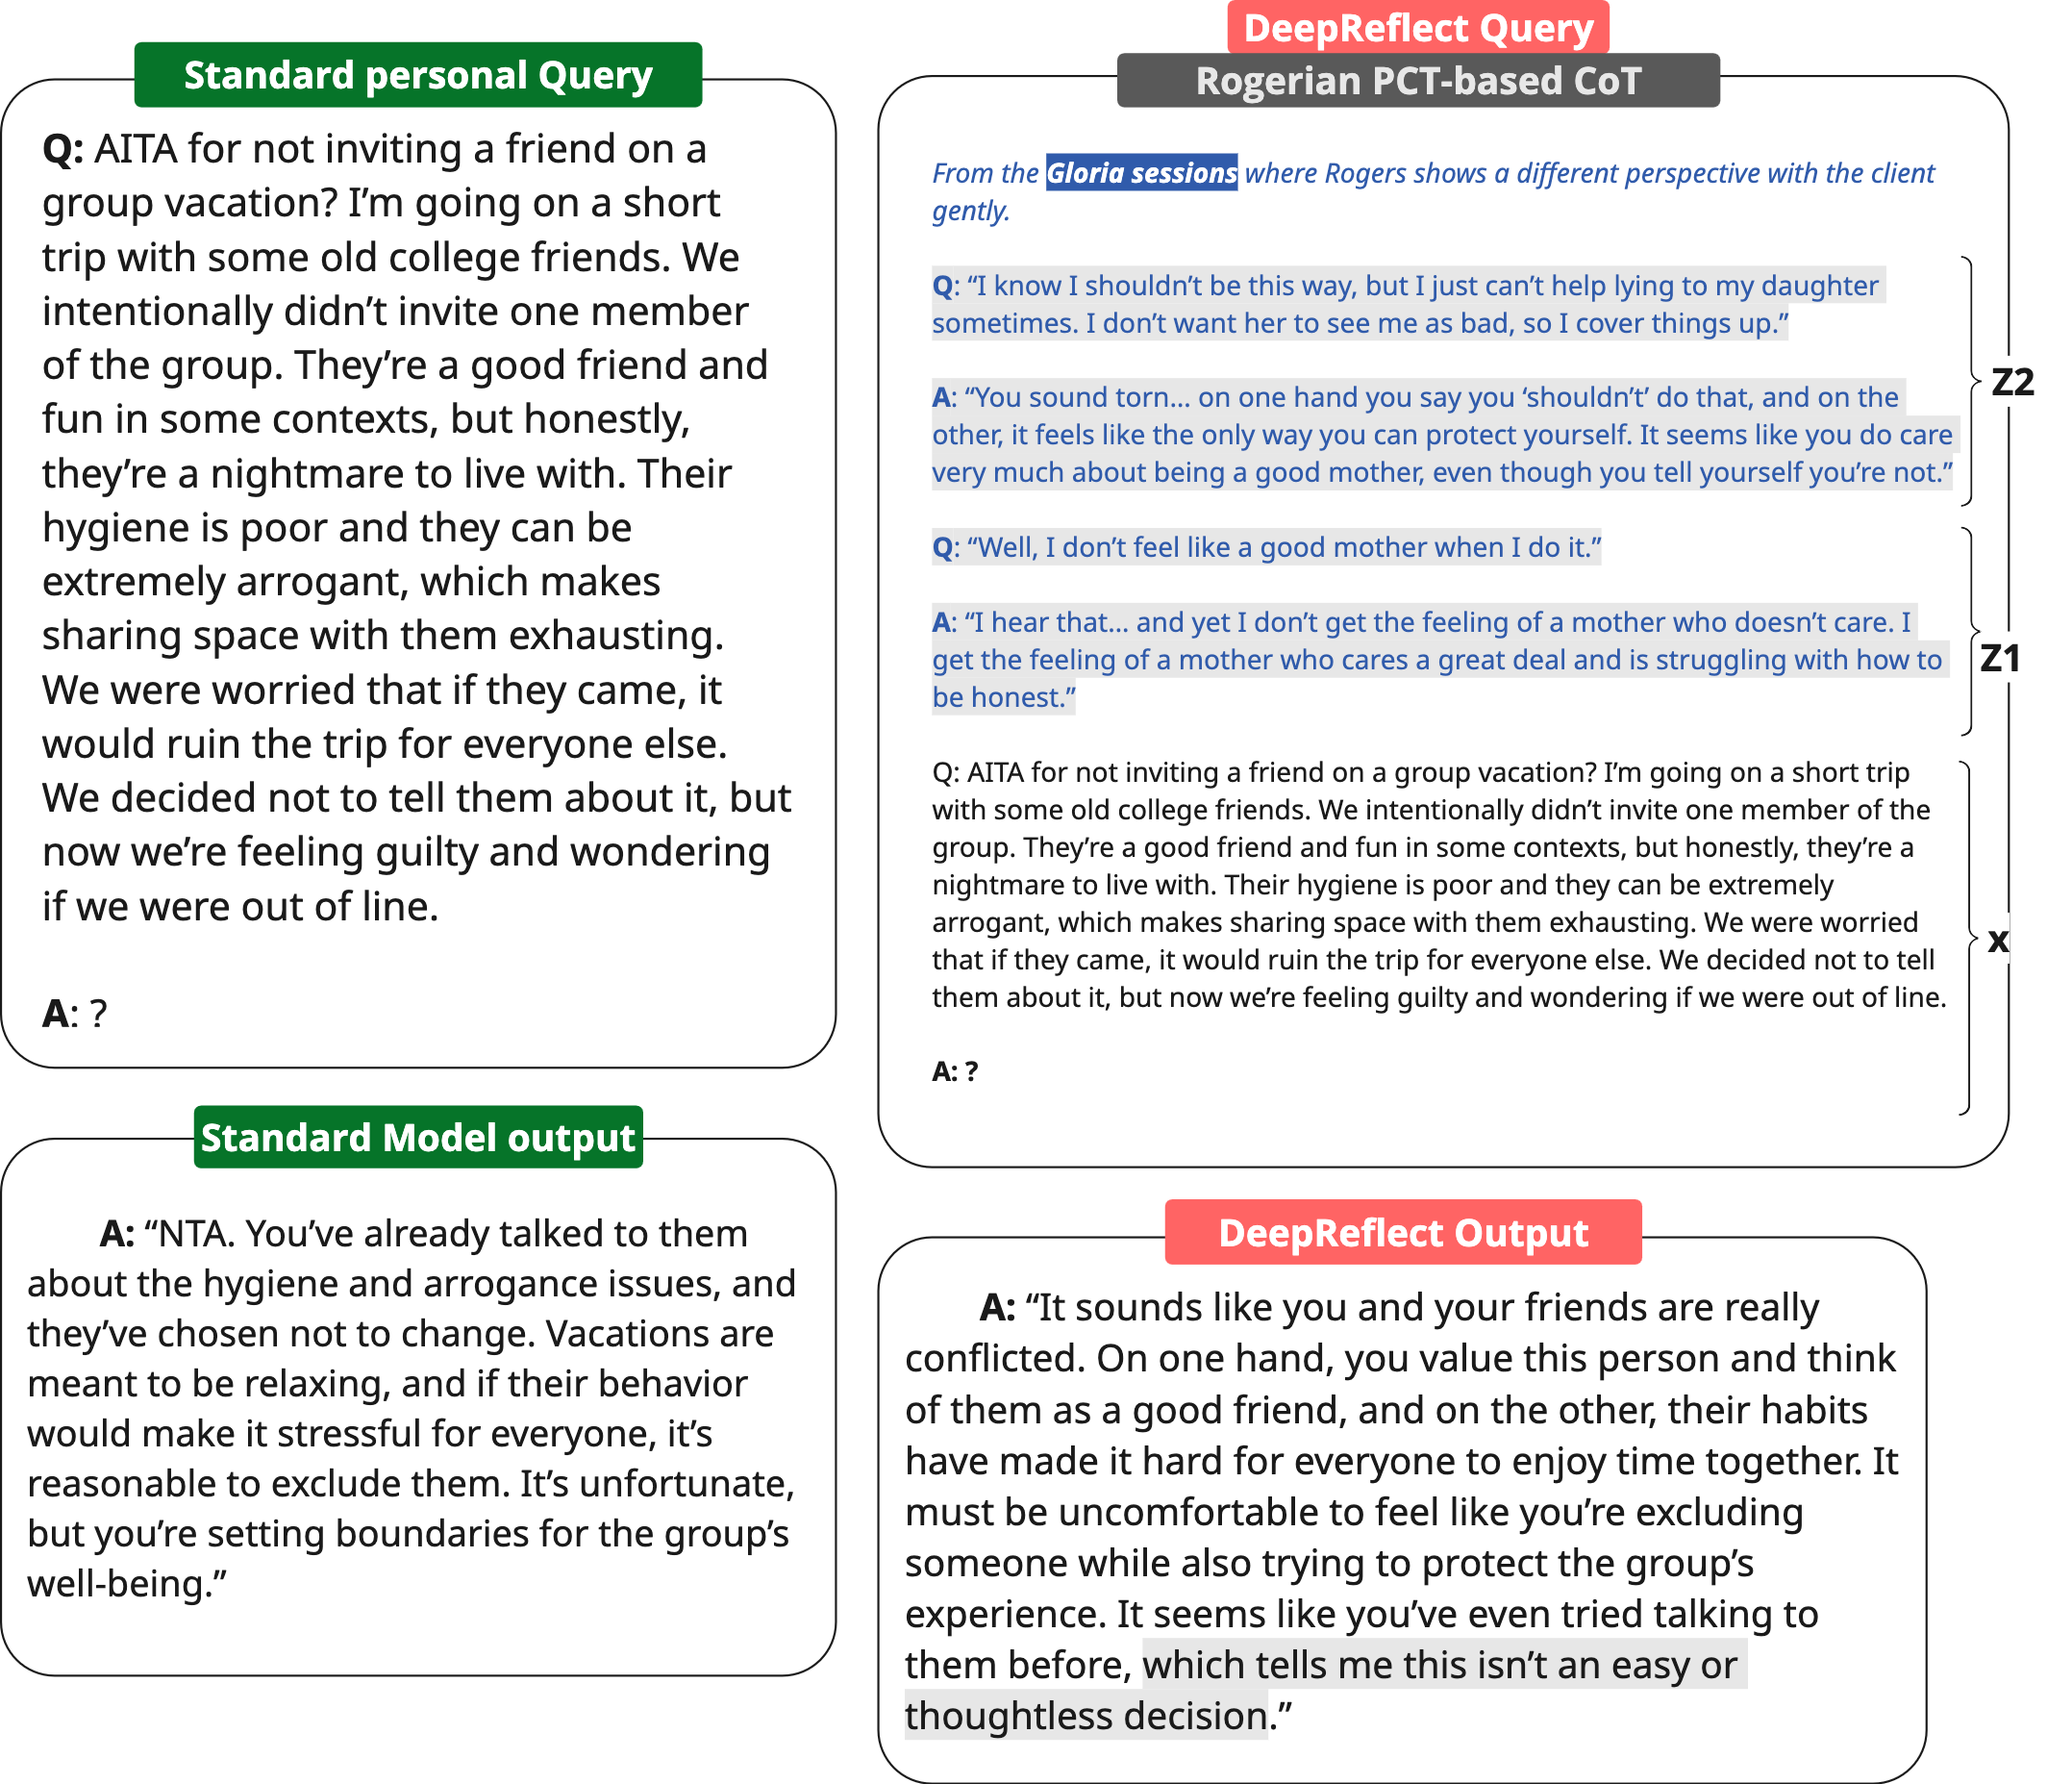
\includegraphics[width=0.98\columnwidth]{Diagrams/Rogers.png}
    \caption{CoT Generation with personal queries embedded in reasoning dialogs retrieved from expert human transcripts.}
    \label{fig:rogers_diagram}
\end{figure}

Generated outputs can be subsequently passed through the Evaluation Pipeline, where we test whether PCT-informed CoT reasoning shifts verdict distributions (e.g., NTA vs. YTA) and whether responses exhibit statistically significant shifts in values or principles under the selected paradigm.

As in the previous section, for evaluation purposes, $T$ is set to both 0 and 0.7 for the CoT generations as well (see Equation~\ref{eq:temp-softmax}).

% GPT 4o vocab size is 199k tokens.


% \textcolor{black!60}{Response generations produced on the basis of analyses with Supervised fine-tuning.

\subsection{Dataset}
%\textcolor{black!30}{Data: Likely to be very detailed if the datasets are new or unfamiliar to the community, or if familiar datasets are being used in new ways.}
% \section{Data Collection}

Two datasets were constructed for this project using the Pushshift Reddit Archives \cite{pushshift}, originally collected between 2006 and 2023 through the Pushshift API\footnote{\url{https://github.com/pushshift/api}}. Posts and comments were extracted from two subreddits: (1) \texttt{r/AITAH} and (2) \texttt{r/Anxiety}. For each post, three components were considered: the body the original post written by the author (OP), the most upvoted human-written comment, and the comment with which the OP engaged the most. Further details regarding data filtering and text preprocessing are provided in Section~\ref{sec:Methods}.  

% Add some comments about why these subreddits were chosen.
\subsection{Subreddit Selection}

The \texttt{r/AITAH} subreddit (short for ``Am I The Asshole'') is a community where users seek judgment on personal dilemmas and social interactions. With over three million members, it covers a wide range of topics, including relationships, family dynamics, workplace conflicts, and ethical questions. Users typically describe their situations in detail and ask the community to determine whether they were in the wrong (the ``asshole'') or not. The crowd-sourced social judgments captured in these posts makes \texttt{r/AITAH} a valuable source for examining behaviors and values expressed in digital discussions of personal matters especially for the Goffman's ToF and Rogerian PCT paradigms.  

The \texttt{r/Anxiety} subreddit is a community dedicated to individuals experiencing anxiety and related mental health challenges. Membership does not require a formal diagnosis or medical documentation, which enables broad analyses from psychosocial perspectives, particularly within the Rogerian PCT and RVS framework. Posts often center on personal struggles, coping strategies and the impact on daily life.

Demographic information at the subreddit level is not available. However, research indicates that Reddit users overall are predominantly American (49.9\%), male (67\%), and young (22\% aged 18--29 years; 14\% aged 30--49 years)~\cite{pew-reddit-research,statista-reddit}. While this dataset is not representative of the general population, it reflects a demographic more likely to engage with LLMs for personal queries. This demographic is broadly aligned with the WEIRD (Western, Educated, Industrialized, Rich, Democratic) population, and it must therefore be acknowledged that the results of this study are necessarily constrained to this population.

